% Options for packages loaded elsewhere
\PassOptionsToPackage{unicode}{hyperref}
\PassOptionsToPackage{hyphens}{url}
%
\documentclass[
]{book}
\usepackage{amsmath,amssymb}
\usepackage{iftex}
\ifPDFTeX
  \usepackage[T1]{fontenc}
  \usepackage[utf8]{inputenc}
  \usepackage{textcomp} % provide euro and other symbols
\else % if luatex or xetex
  \usepackage{unicode-math} % this also loads fontspec
  \defaultfontfeatures{Scale=MatchLowercase}
  \defaultfontfeatures[\rmfamily]{Ligatures=TeX,Scale=1}
\fi
\usepackage{lmodern}
\ifPDFTeX\else
  % xetex/luatex font selection
\fi
% Use upquote if available, for straight quotes in verbatim environments
\IfFileExists{upquote.sty}{\usepackage{upquote}}{}
\IfFileExists{microtype.sty}{% use microtype if available
  \usepackage[]{microtype}
  \UseMicrotypeSet[protrusion]{basicmath} % disable protrusion for tt fonts
}{}
\makeatletter
\@ifundefined{KOMAClassName}{% if non-KOMA class
  \IfFileExists{parskip.sty}{%
    \usepackage{parskip}
  }{% else
    \setlength{\parindent}{0pt}
    \setlength{\parskip}{6pt plus 2pt minus 1pt}}
}{% if KOMA class
  \KOMAoptions{parskip=half}}
\makeatother
\usepackage{xcolor}
\usepackage{longtable,booktabs,array}
\usepackage{calc} % for calculating minipage widths
% Correct order of tables after \paragraph or \subparagraph
\usepackage{etoolbox}
\makeatletter
\patchcmd\longtable{\par}{\if@noskipsec\mbox{}\fi\par}{}{}
\makeatother
% Allow footnotes in longtable head/foot
\IfFileExists{footnotehyper.sty}{\usepackage{footnotehyper}}{\usepackage{footnote}}
\makesavenoteenv{longtable}
\usepackage{graphicx}
\makeatletter
\def\maxwidth{\ifdim\Gin@nat@width>\linewidth\linewidth\else\Gin@nat@width\fi}
\def\maxheight{\ifdim\Gin@nat@height>\textheight\textheight\else\Gin@nat@height\fi}
\makeatother
% Scale images if necessary, so that they will not overflow the page
% margins by default, and it is still possible to overwrite the defaults
% using explicit options in \includegraphics[width, height, ...]{}
\setkeys{Gin}{width=\maxwidth,height=\maxheight,keepaspectratio}
% Set default figure placement to htbp
\makeatletter
\def\fps@figure{htbp}
\makeatother
\setlength{\emergencystretch}{3em} % prevent overfull lines
\providecommand{\tightlist}{%
  \setlength{\itemsep}{0pt}\setlength{\parskip}{0pt}}
\setcounter{secnumdepth}{5}
\usepackage{booktabs}
\usepackage{amsthm}
\makeatletter
\def\thm@space@setup{%
  \thm@preskip=8pt plus 2pt minus 4pt
  \thm@postskip=\thm@preskip
}
\makeatother
\ifLuaTeX
  \usepackage{selnolig}  % disable illegal ligatures
\fi
\usepackage[]{natbib}
\bibliographystyle{apalike}
\IfFileExists{bookmark.sty}{\usepackage{bookmark}}{\usepackage{hyperref}}
\IfFileExists{xurl.sty}{\usepackage{xurl}}{} % add URL line breaks if available
\urlstyle{same}
\hypersetup{
  pdftitle={AI Tools in the Job Recruiting Process},
  pdfauthor={Jingyi (Vera) Wang, Kuigang (KG) Zhang, Michael Czapp, Xinqian (Demi) Dai, Yousuf Altameemi},
  hidelinks,
  pdfcreator={LaTeX via pandoc}}

\title{AI Tools in the Job Recruiting Process}
\author{Jingyi (Vera) Wang, Kuigang (KG) Zhang, Michael Czapp, Xinqian (Demi) Dai, Yousuf Altameemi}
\date{2023-08-09}

\begin{document}
\maketitle

{
\setcounter{tocdepth}{1}
\tableofcontents
}
\hypertarget{introduction-to-our-book}{%
\chapter{Introduction to Our Book}\label{introduction-to-our-book}}

For students at the Stephen M. Ross School of Business, the primary goal by graduation is to have a full-time job offer at a company and location that makes them excited to start their professional careers. Throughout the fall and winter semesters, recruiting is an incredibly time-consuming and stressful process, so students must use their time and effort efficiently to maximize their job opportunities. However, the recent and rapid progression of artificial intelligence (AI) tools has reshaped the recruiting landscape. Therefore, students need to understand how they can use these tools to their advantage and how recruiters may be using AI throughout the recruitment process.

Our book will provide a comprehensive overview of these AI tools. We will approach this from two perspectives: students' and recruiters'. For students, we discuss how they can use AI job finders, resume and cover letter optimization, practice interviews, and automated applications to support their professional endeavors. On the other hand, we discuss what AI tools recruiters may use, like applicant tracking systems (ATS), resume and cover letter screening, interview assessments, skill assessments, and predictive analytics. Then, we suggest how students should tailor their presentation of themselves to fit what these AI tools look for.

\hypertarget{about-us}{%
\chapter{About Us}\label{about-us}}

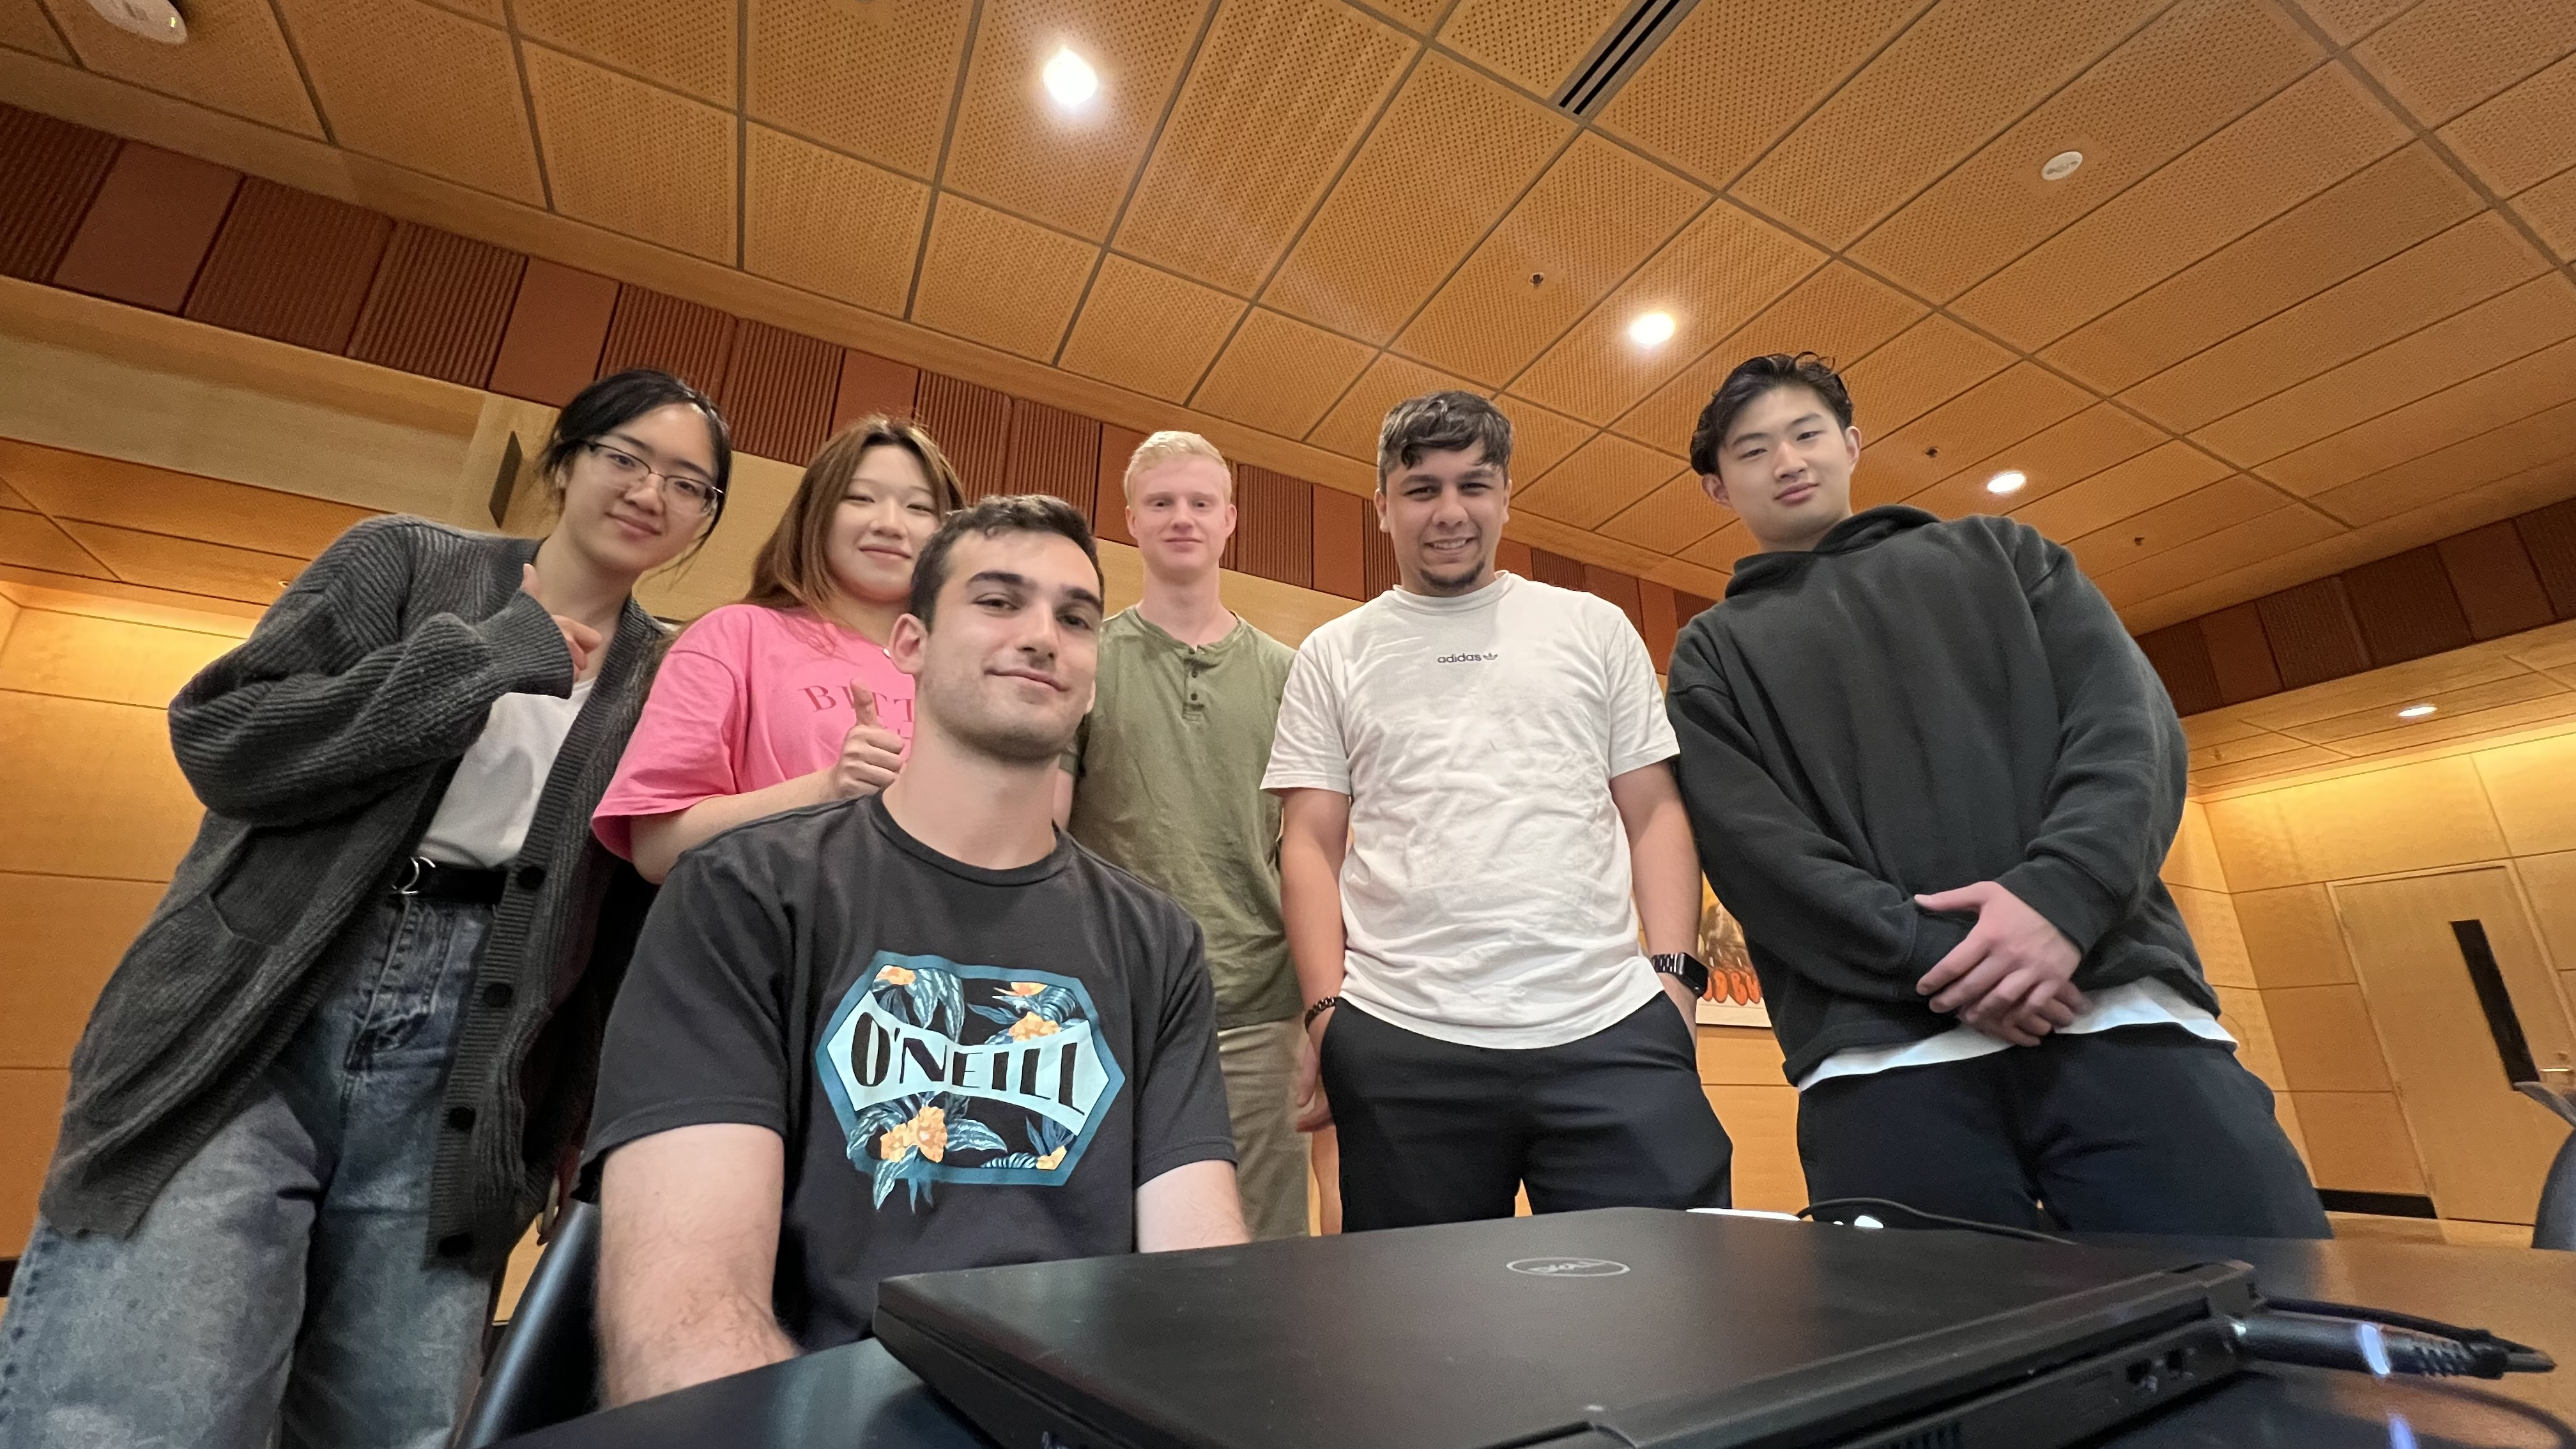
\includegraphics[width=4.04167in,height=\textheight]{Team Photo.jpg}

Our team, \textbf{Team Steve}, is driven by Steve's desire for a website that describes how new AI Tools are used in the recruitment process. For context, Steve (as seen in the black O'Neill shirt in the front left) is a student here at the Stephen M. Ross School of Business who is NOT in our project team. When deciding our team name, we thought it'd be a great idea to name it after the first person we encounter. We happened to run into Steve outside of our classroom, and the rest is history.

\hypertarget{jingyi-wang}{%
\section{Jingyi Wang}\label{jingyi-wang}}

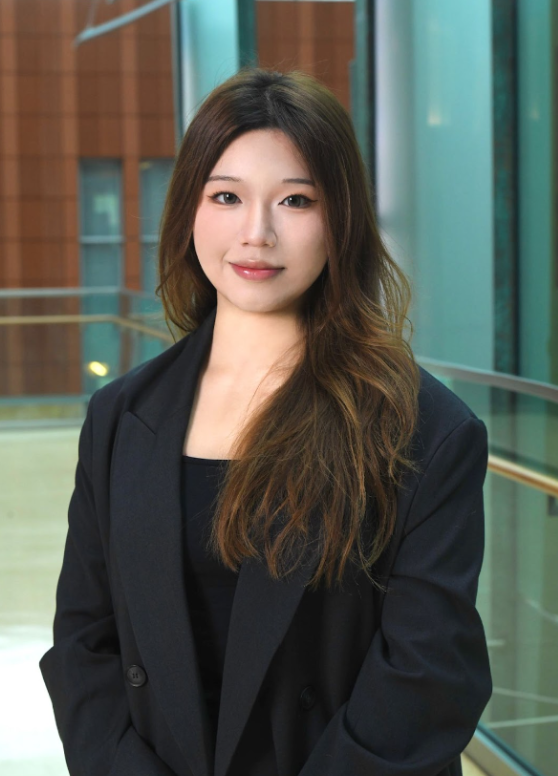
\includegraphics[width=2.16667in,height=\textheight]{Vera Photo.png}

\textbf{Background}

My name is Jingyi (Vera) Wang, currently a Master of Business Analytics student at the University of Michigan Ross School of Business. In May 2023, I graduated from Boston University with a concentration in Finance and Business Analytics. From my previous academic and internship experiences, I found my passion for business analytics. That's the reason why I decided to pursue a graduate degree in order to help me specialize in my area of interest and enrich my experience and knowledge in the field.

\textbf{Experience}

My experience is mainly composed of internships, projects, and case competitions. In 2021, I interned at Accenture as a management consulting intern. I managed project plans, conducted data analysis, and facilitated platform testing sessions for clients to improve the efficiency and accuracy of their online platform. In 2022, I interned at Vantage House Media as a finance intern. I generated comprehensive financial reports and provided stakeholders with valuable recommendations and potential VC prospects based on data analysis. In addition, I was a quantitative financial analyst intern at Shenwan Hongyuan Securities, where I built python models to select top-performing stocks and assess fund managers' performance.~

\textbf{Fun Facts}

\begin{itemize}
\item
  I have two pet guinea pigs
\item
  I never watch horror movies
\item
  I love photography, and I have previously operated a photography social account of my own
\end{itemize}

\hypertarget{kuigang-zhang}{%
\section{Kuigang Zhang}\label{kuigang-zhang}}

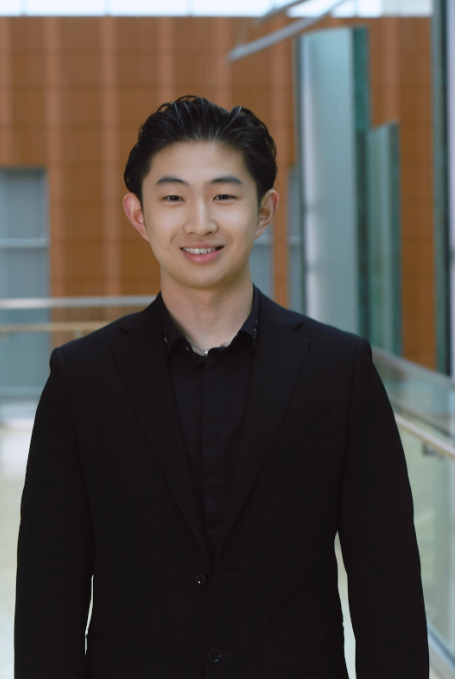
\includegraphics[width=2.1875in,height=\textheight]{KG Photo.png}

\textbf{Background}

My name is Kuigang Zhang, and I go by KG. I graduated from UCLA with a Data Science major and an Accounting minor in June 2023. Programming and business have been two areas that I am passionate about; therefore, I decided to pursue a Master of Business Analytics here at the University of Michigan Ross School of Business. I look forward to enriching my toolbox, meeting like-minded people, and getting the most out of the program.

\textbf{Experience}

I have four years of experience in programming, and have completed a number of Kaggle Competition as well as machine learning projects, and I have worked as an data analyst intern at the Shanghai Research Institute of Building Science Academy, where I enabled household energy consumption forecast in Shanghai for managing and planning urban energy utilization, covering a wide range of locations and building types.I have also worked as a data analyst intern at Lin Zhen Trading, where I developed an integrated data-driven retail supply chain management app in support of the bedding items business.

\textbf{Fun Facts}

\begin{itemize}
\item
  I was born and raised in Africa
\item
  I can deadlift 400lbs
\item
  I speak 5 languages
\end{itemize}

\hypertarget{michael-czapp}{%
\section{Michael Czapp}\label{michael-czapp}}

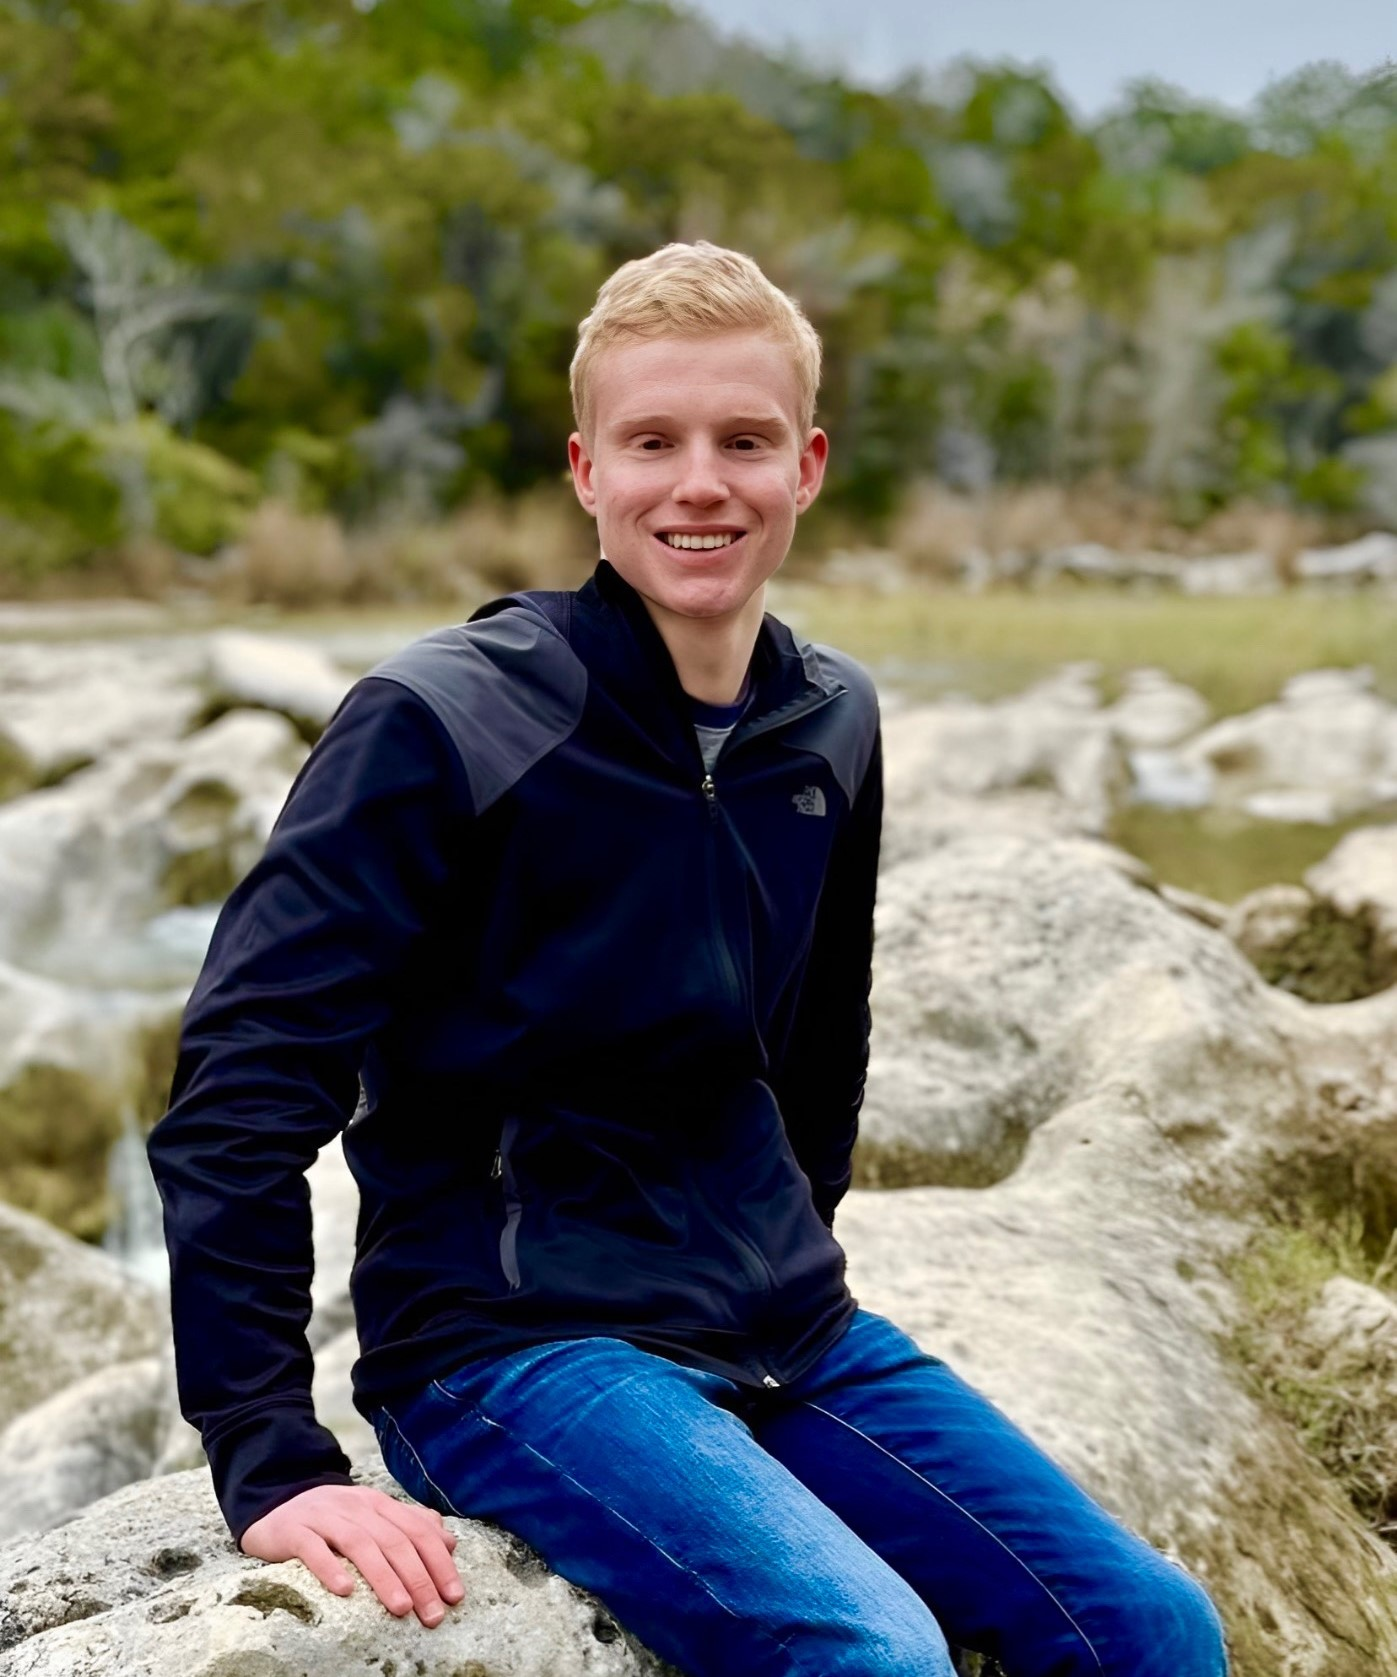
\includegraphics[width=2.36458in,height=\textheight]{Michael Czapp Photo.jpeg}

\textbf{Background}

My name is Michael Czapp, and I am currently a Master of Business Analytics (MBAn) student at the University of Michigan Ross School of Business. In April 2023, I graduated from the College of Engineering here with a Bachelor of Science in Industrial \& Operations Engineering. I knew I wanted to specialize in analytics, so starting a graduate program right after graduation made the most sense. It also allowed me to have an extra year at the University of Michigan and stay in my home state, and I plan to make the most of it!

\textbf{Experience}

My experience primarily consists of two summer internships. In 2021, I interned at DTE Energy in Detroit, MI as a Continuous Improvement Intern. I got to develop Power BI dashboards, lead a time study analysis on claim investigations, and support the execution of a pilot study at one of the company's sites. In 2022, I interned at Boston Scientific Corporation as a Global Supply Chain Consulting Intern, which was essentially an internal consulting role. I built automations, helped plan a global virtual conference, and used Excel to identify opportunities to decrease shipping costs to customers, all of which provided me with great experience in using data to discover meaningful insights to share with stakeholders.

\textbf{Fun Facts}

\begin{itemize}
\item
  Both my older brother and sister studied industrial engineering in undergrad
\item
  I play hockey as both a goalie and a skater
\item
  I've lived in the state of Michigan for my entire life
\end{itemize}

\hypertarget{xinqian-dai}{%
\section{Xinqian Dai}\label{xinqian-dai}}

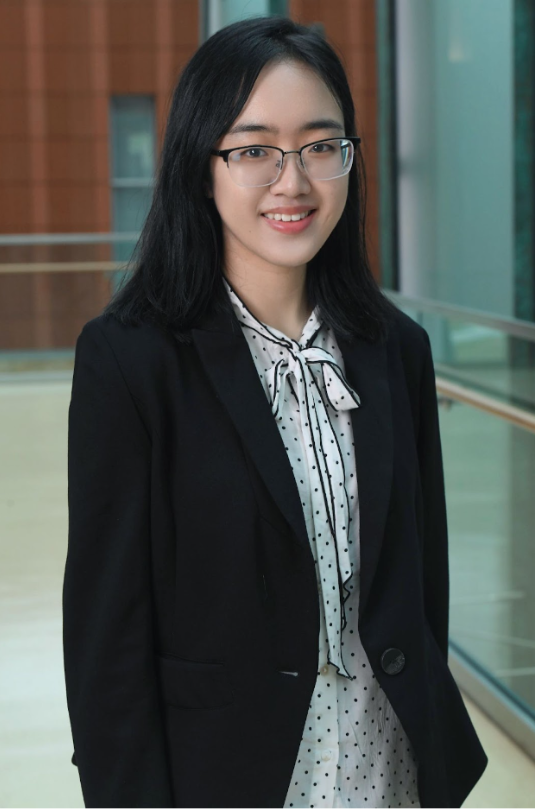
\includegraphics[width=2.08333in,height=\textheight]{Demi Photo.png}

\textbf{Background}

Hello! My name is Xinqian (Demi) Dai, and I come from the beautiful province of Heilongjiang, China, where I was born and raised. In 2019, I embarked on my exciting journey by enrolling at the University of Massachusetts Amherst for my undergraduate studies. I graduated with a double major in Marketing and Statistics in May 2023. My interest in Marketing has deep roots that extend back to my childhood days when I found myself more fascinated by the commercial inserts of a washing powder than the animated series on TV.~ Currently, I am intrigued by Customer Analytics, Advertising Effectiveness, and Digital Marketing, and I'm eager to delve deeper into these areas. Looking ahead, my post-graduation aspirations involve entering into the MarTech (Marketing Technology) industry. Armed with the knowledge and skills from the MBAn program, I aim to make a significant impact by applying data-driven strategies and innovative marketing technologies.

\textbf{Experience}

During my time at UMass Amherst, I engaged in a diverse range of research experiences and marketing projects. As a Marketing Research Assistant at the UMass Ombuds Office, I analyzed data from over 300 undergraduate student visitors, studying variables like gender and major to identify successful conflict resolution strategies. Utilizing R and Python, I applied regression models to estimate meeting times and understand the impact of visitor demographics on appointment durations. During my participation in the Research Experiences for Undergraduates (REU) Program, I conducted full-time research on Bayesian parameter estimations, highlighting the effectiveness of Bayesian models over traditional linear regression models. Additionally, as a Research Assistant in the UMass Marketing Department, I analyzed customer reactions to visual advertisements for various product categories and conducted experiments to evaluate the effect of different headbands on students. As a Strategist for the UMass AdLab, I designed customized questionnaires and implemented successful advertising strategies, resulting in a significant increase in orders for local companies. These experiences have shaped my passion for business analytics and my dedication to data-driven research and strategic planning.

\textbf{Fun Facts}

\begin{itemize}
\item
  A24 is my favorite film production company
\item
  I'm better at cooking than baking:))
\item
  My hometown holds the International Ice and Snow Festival every winter
\end{itemize}

\hypertarget{yousuf-altameemi}{%
\section{Yousuf Altameemi}\label{yousuf-altameemi}}

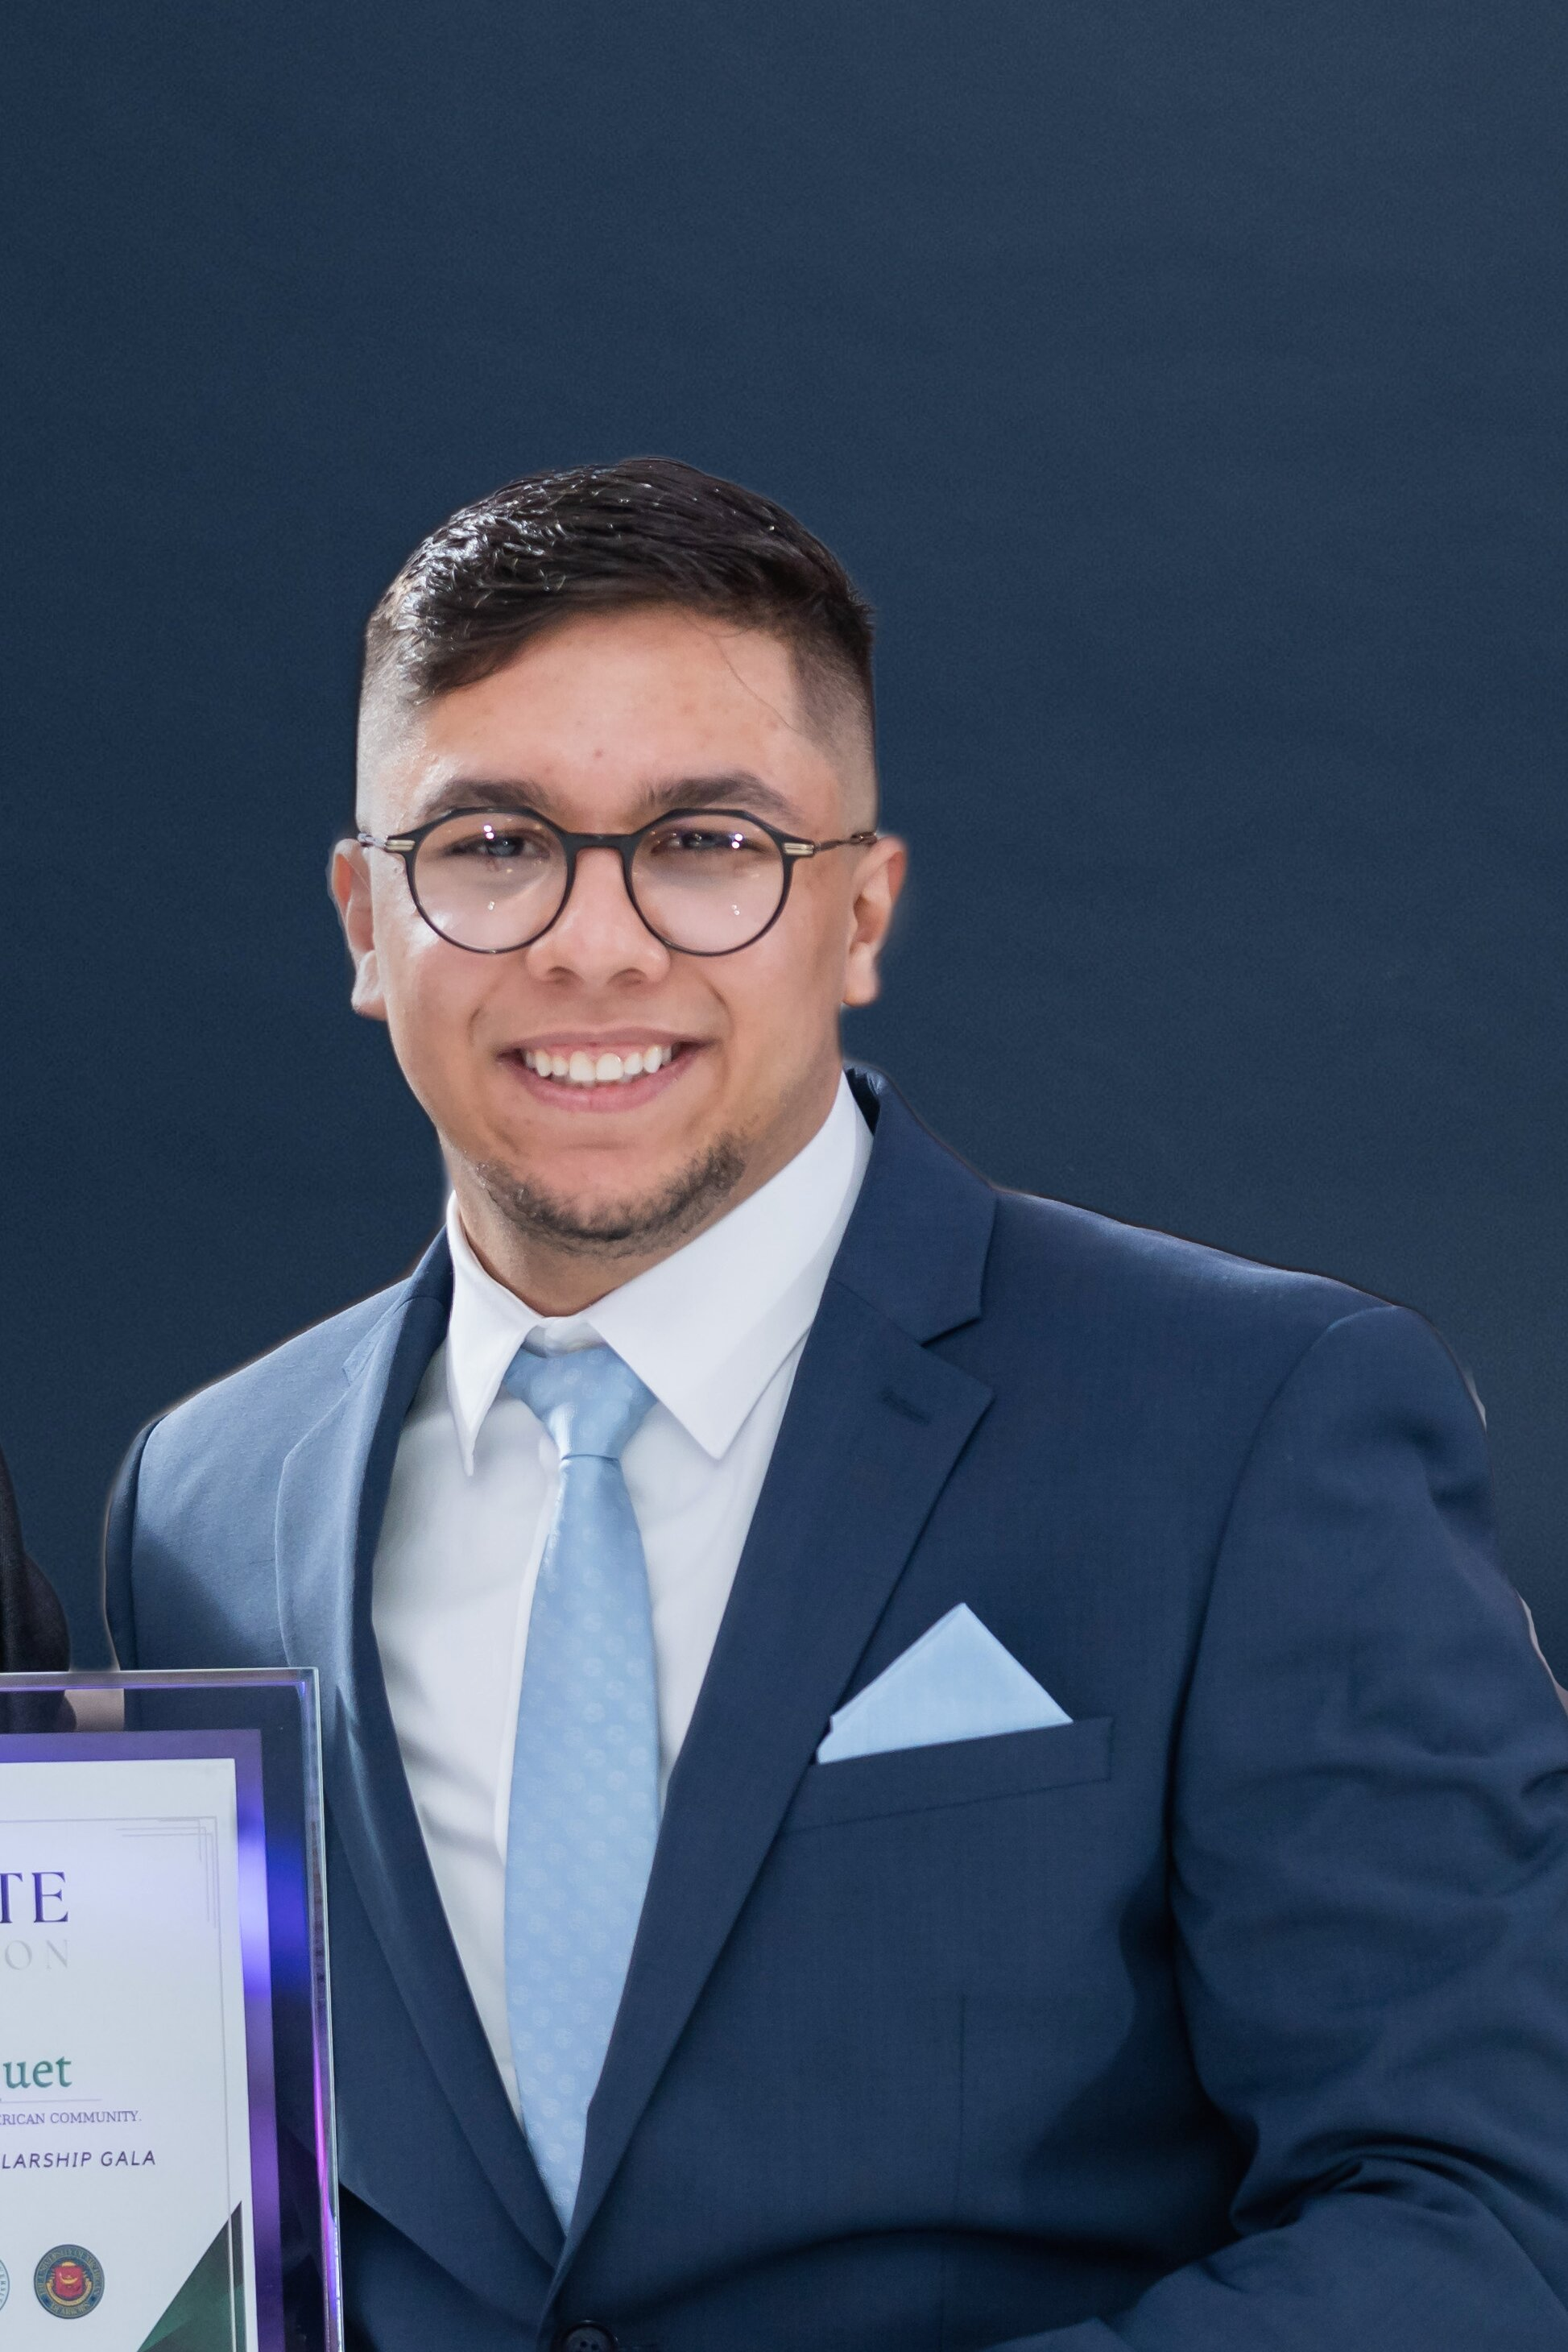
\includegraphics[width=2.38542in,height=\textheight]{Headshot.jpg}

\textbf{Background}

I was born and raised in Baghdad, Iraq, but now I live in the metro Detroit area. Besides my regular job, I love doing photography as a hobby. I enjoy capturing moments and emotions with my camera, and it lets me see the world in a whole new way. Additionally, I have a knack for analytics; I enjoy working with data, finding patterns, and gaining valuable insights from it. This analytical mindset helps me both in my photography and other aspects of life.

\textbf{Experience}

I graduated from Wayne State University in 2022 with a double major in Finance and Business Administration. For the past three years, I have been working as an IT Business Analyst at DTE Energy, where I have been involved in various analytical projects within the IT department. My responsibilities include analyzing data, identifying patterns, and providing valuable insights that contribute to the company's IT strategies and decision-making processes. I have also had the opportunity to collaborate with external consultants, showcasing my ability to work effectively with diverse teams and stakeholders. With a strong analytical mindset and a background in finance and business, I am well-equipped to contribute positively to any project or team I am a part of.

\textbf{Fun Facts}

\begin{itemize}
\item
  I am a part-time photographer, I shoot portraits, events and weddings
\item
  I enjoy playing soccer, my friends and I play twice a week
\item
  I collect vintage Ralph Lauren clothing
\end{itemize}

\hypertarget{what-is-artificial-intelligence-ai}{%
\chapter{What is Artificial Intelligence (AI)?}\label{what-is-artificial-intelligence-ai}}

Artificial intelligence is the simulation of human intelligence processes by machines, especially computer systems. Specific applications of AI include expert systems, natural language processing, speech recognition and machine vision (1).

The functioning of AI involves the processing of extensive labeled training data, identifying correlations and patterns within the data, and using these patterns to make predictions about future states. For instance, a chatbot can learn to produce lifelike conversations with people after being trained on text examples, while an image recognition tool can accurately identify and describe objects in images through the analysis of millions of examples. Generative AI techniques have also shown significant progress in generating realistic text, images, music, and other media.

AI programming revolves around cognitive skills that encompass:

\textbf{1. Learning}: The acquisition of data and creation of algorithms that convert it into actionable information, providing step-by-step instructions for specific tasks to computing devices.

\textbf{2. Reasoning:} The selection of appropriate algorithms to achieve desired outcomes.

\textbf{3. Self-correction:} Continuously refining algorithms to ensure optimal and precise results.

\textbf{4. Creativity:} Utilizing neural networks, rules-based systems, statistical methods, and other AI techniques to generate novel images, text, music, and ideas.

The significance of artificial intelligence lies in its potential to revolutionize how we live, work, and engage in leisure activities. AI has found effective applications in automating tasks traditionally performed by humans, such as customer service, lead generation, fraud detection, and quality control. Particularly in repetitive and detail-oriented tasks, AI often outperforms humans in terms of speed and accuracy, as demonstrated in analyzing vast numbers of legal documents for accurate field completion. The processing capabilities of AI enable enterprises to gain valuable insights into their operations that were previously inaccessible.

The proliferation of AI tools, especially generative AI, promises transformative impacts across various domains, including education, marketing, and product design. Leading companies like Alphabet, Apple, Microsoft, and Meta have integrated AI technologies to enhance their operations and maintain a competitive edge. For instance, Google, a subsidiary of Alphabet, employs AI at the core of its search engine, Waymo's self-driving cars, and Google Brain, the pioneer behind the transformer neural network architecture that drives recent advancements in natural language processing.

Overall, the advent of AI not only drives efficiency improvements but also creates unprecedented business opportunities, as evidenced by Uber's success in leveraging computer software to connect riders with taxis and becoming a Fortune 500 company. The ongoing progress in AI holds the potential to shape a dynamic and transformative future across various industries.

\hypertarget{ai-tools-for-job-searching}{%
\chapter{AI Tools for Job Searching}\label{ai-tools-for-job-searching}}

\hypertarget{resume-and-cover-letter-optimizers}{%
\chapter{Resume and Cover Letter Optimizers}\label{resume-and-cover-letter-optimizers}}

In today's competitive and ever-changing job market, it is crucial to have a well-crafted resume and cover letter to stand out from competitors and gain the opportunity to catch employers' attention. With the recent advancements in AI tools, students can now leverage technology to optimize their resumes and cover letters effectively. Here are some popular AI resume and cover letter builders:

\hypertarget{resume.com}{%
\section{Resume.com}\label{resume.com}}

\href{https://www.resume.com/resume/builder/783ccdad-f0ea-4ff0-aa57-c59d6100995a}{Resume.com} is a free online resume builder that helps you create a resume tailored to your skills and experience. One outstanding feature of Resume.com is to pinpoint the most relevant keywords for your target positions to mention in the resume, which is essentially beneficial when applying for positions that require specific technical or professional skills and abilities. In addition, it also provides various customizable templates, editing tools, resume tips, and resume sample, where you could easily edit your content based on your individual needs. It also provides a resume evaluation service by giving personalized feedback on your resume.

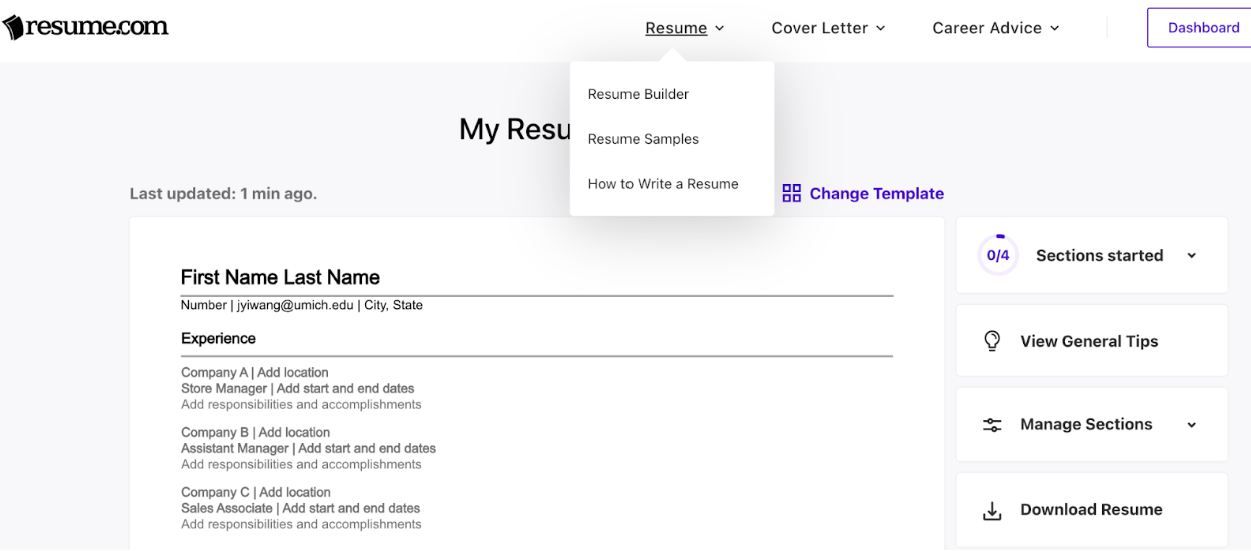
\includegraphics[width=5.90625in,height=\textheight]{Resume.com pic.png}

\hypertarget{jobscan}{%
\section{Jobscan}\label{jobscan}}

\href{https://www.jobscan.co/resume-score}{Jobscan} is a popular AI resume builder that analyzes your resume and provides suggestions for improvements based on the description and keyword. It has the unique feature of scanning a resume against a specific job description, offering you a detailed report about how your skills and experience are being matched with areas where you can enhance your alignment with the role. It provides a very detailed feedback report showcasing which section you should focus on by listing out your missing skills and keywords for several sections: ATS findings, recruiter findings, hard skills, and soft skills.

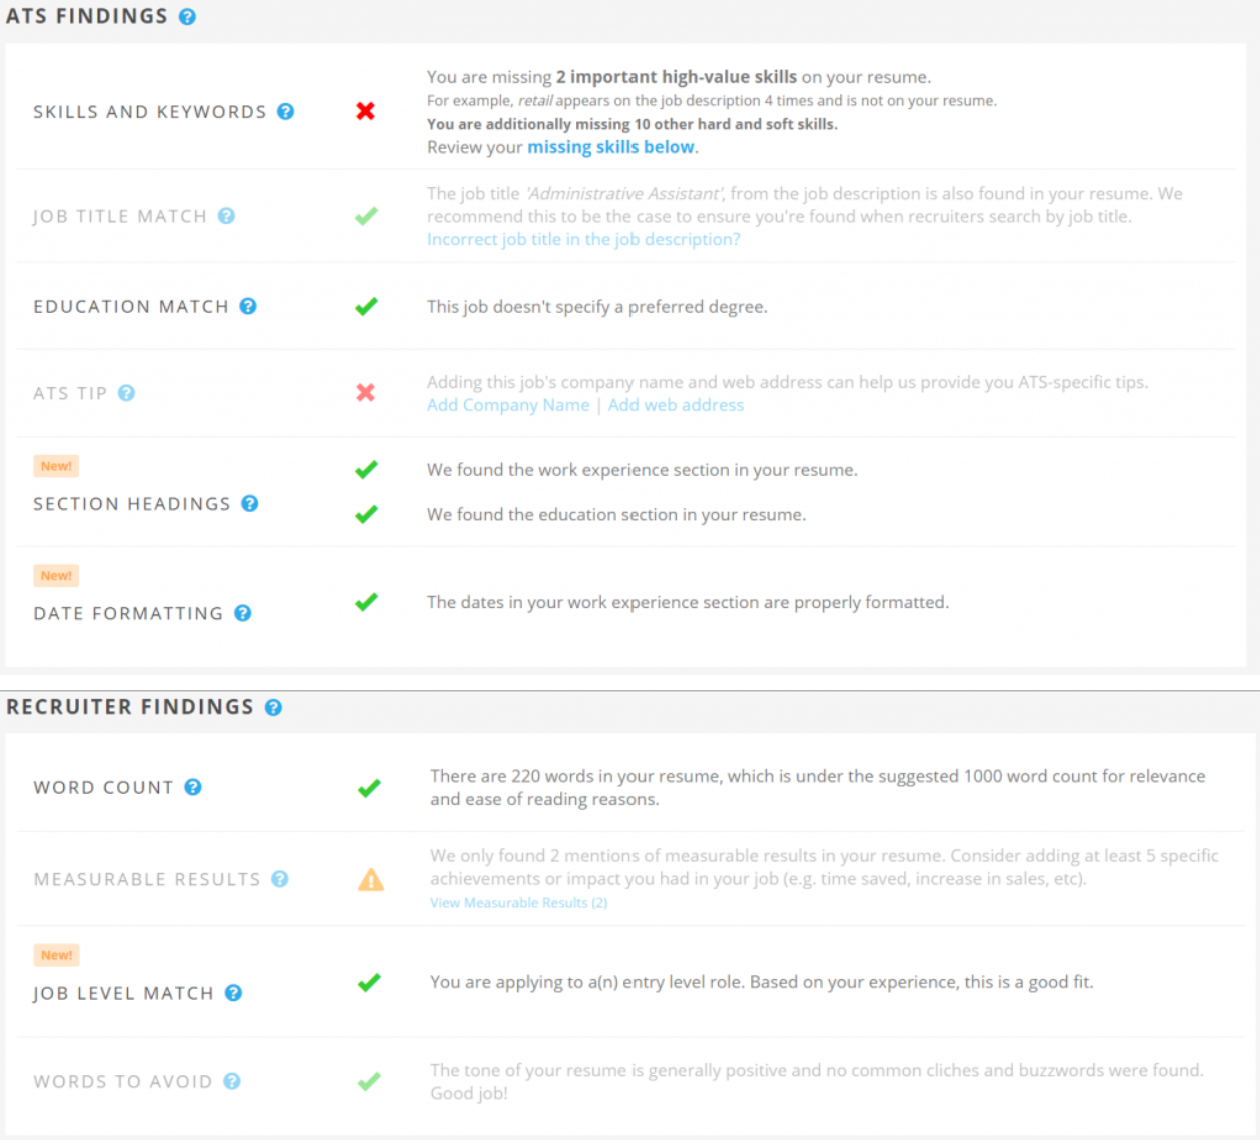
\includegraphics[width=5.11458in,height=\textheight]{Jobscan findings.png}

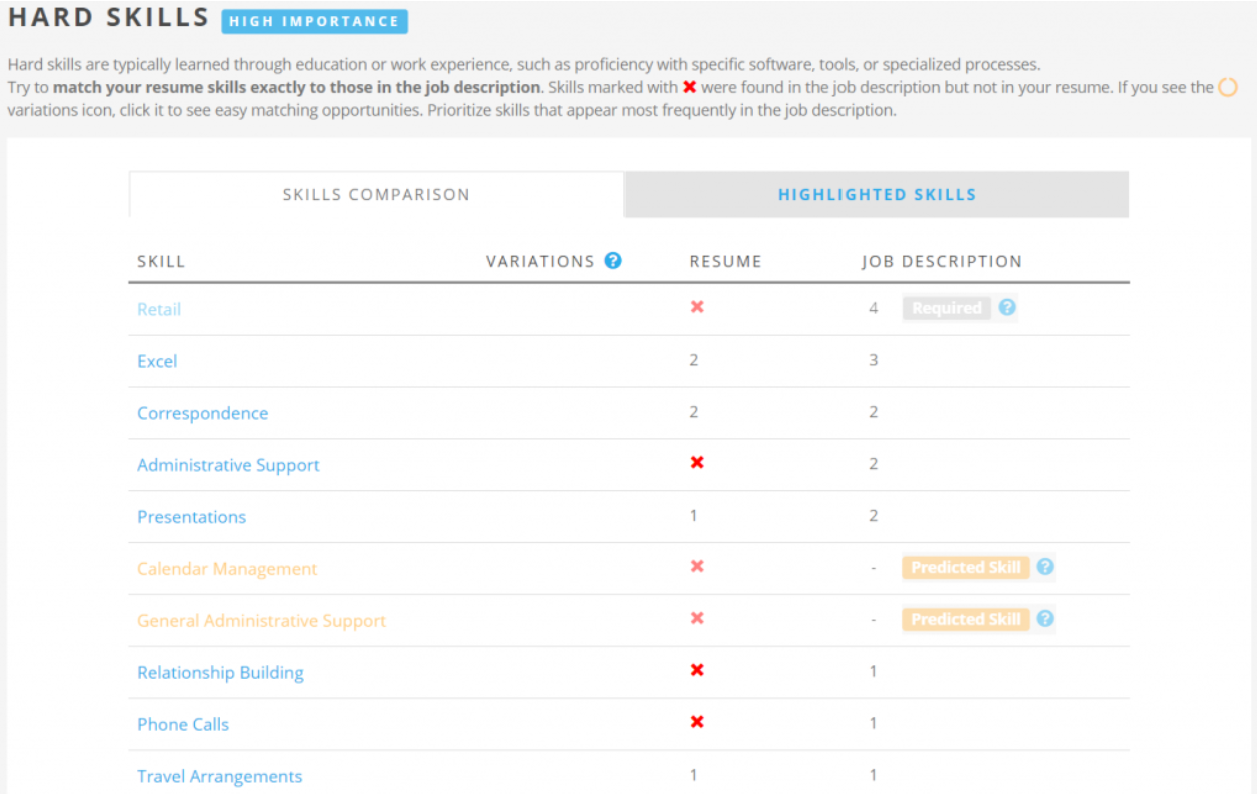
\includegraphics[width=3.98958in,height=\textheight]{Jobscan findings 2.png}

\hypertarget{kickresume}{%
\section{Kickresume}\label{kickresume}}

The modern AI resume builder \href{https://www.kickresume.com/en/}{Kickresume} makes the process from creating to checking a resume much easier than before. It includes a wide range of designer-created templates, a detail-oriented log of changes made to your resume, a drag-and-drop editor, and a easy-to-use one-click design feature. It generates and optimizes well-formatted professional resumes that strongly match with your personalized positions by utilizing various in-build AI tools such as spell checkers, AI text analysis, natural language processing, and style guides. In addition, Kickresume offers an unique feature that allows users to upload a video introduction as an alternative job submission method instead of traditional resume format. This video can help employers better understand your strengths and skills. All these features make Kickresume a great platform for job seekers to improve their professional credentials and create a high-quality resume in a short amount of time.

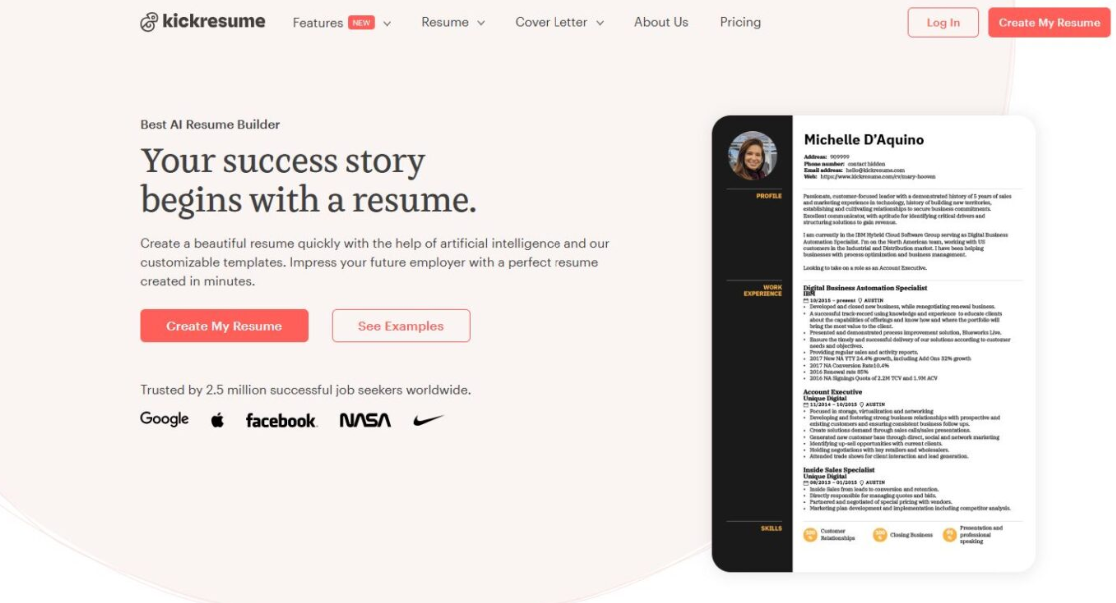
\includegraphics[width=5.46875in,height=\textheight]{Kickresume pic.png}

\hypertarget{lazyapply}{%
\section{LazyApply}\label{lazyapply}}

\href{https://lazyapply.com/cover-letter-generator}{LazyApply} is a free AI cover letter generator to help you create professional cover letters easily. It includes over 20 options of writing tones, such as humble, convincing, appreciative, formal, and inspirational, to assist you with generating the most suitable writing style for your personal cover letter. By simply inputting your personal details like your name, skills, the job information, and the recruiter's name to whom you want to send the cover letter, it helps you generate an appropriate cover letter fast and accurately. Moreover, it offers abundant cover letter templates based on specific organizations or job roles, such as Amazon cover letter and Product Manager cover letter.

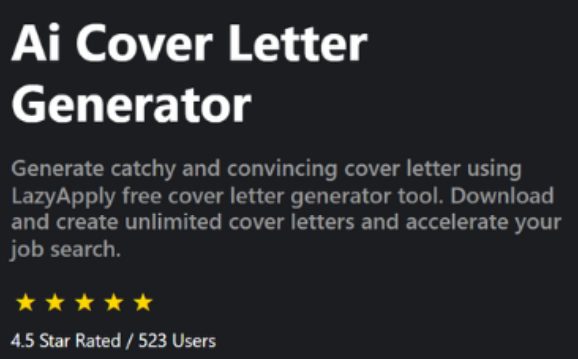
\includegraphics[width=3.59375in,height=\textheight]{Lazyapply pic.png}

\hypertarget{rezi}{%
\section{Rezi}\label{rezi}}

\href{https://www.rezi.ai/}{Rezi} is a professional AI cover letter generator. It provides over 250+ cover letter samples, which allows job seekers to begin the process of creating cover letters. After analyzing your resume, Rezi makes references from your resume experiences and how they fit best for the job role in your cover letter. If you enter the ideal company details and specific skills and position highlights, Rezy will generate a tailored cover letter in seconds.~

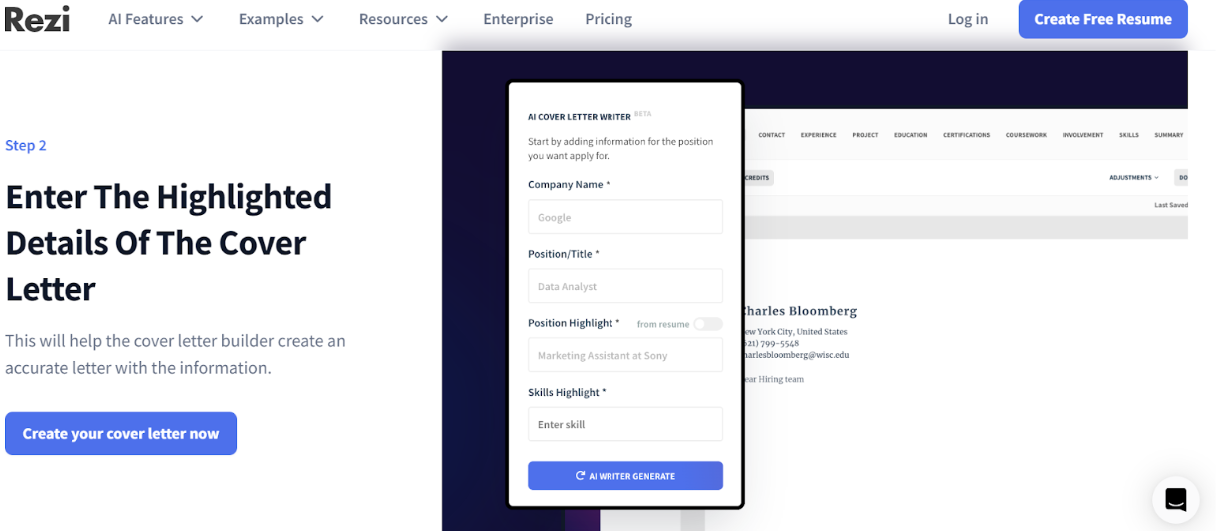
\includegraphics[width=5.5in,height=\textheight]{Rezi pic.png}

\hypertarget{cover-letter-simple.ai}{%
\section{Cover Letter Simple.ai}\label{cover-letter-simple.ai}}

\href{https://coverlettersimple.ai/}{Cover Letter Simple.ai} is unique from other cover letter tools mentioned above as it focuses on generating unique and job-specific cover letters. After entering your ideal job title, it searches billions of data points to retrieve relevant information for the job, such as expected skills and accomplishments. It then generates impressive cover letters that help you stand out from other applicants.

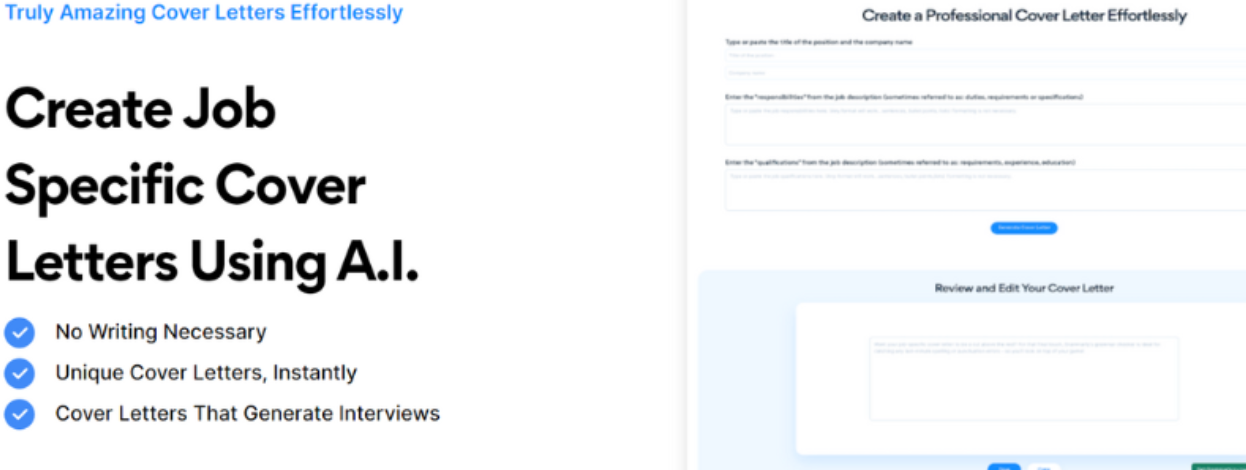
\includegraphics[width=6.80208in,height=\textheight]{coverlettsimpleai pic.png}

\hypertarget{student-practice-interviews}{%
\chapter{Student Practice Interviews}\label{student-practice-interviews}}

\hypertarget{automated-applications}{%
\chapter{Automated Applications}\label{automated-applications}}

\hypertarget{what-are-applicant-tracking-systems-ats}{%
\chapter{What Are Applicant Tracking Systems (ATS)?}\label{what-are-applicant-tracking-systems-ats}}

\hypertarget{recruiting-chatbots}{%
\chapter{Recruiting Chatbots}\label{recruiting-chatbots}}

\hypertarget{resume-and-cover-letter-screening}{%
\chapter{Resume and Cover Letter Screening}\label{resume-and-cover-letter-screening}}

\hypertarget{video-interview-assessments}{%
\chapter{Video Interview Assessments}\label{video-interview-assessments}}

One way that recruiters may also quicken the recruitment process is to use AI tools that analyze video interviews, whether self-recorded by the candidate or from an actual interview with employees from the company. More commonly, though, the video interview assessment that an AI conducts will be through a self-recorded interview the candidate will record on the employer's hiring platform. \textbf{Watch the following video for a concise summary of how AI can be used in the interview process!}

\href{https://www.youtube.com/watch?v=cJkHft032OE}{The AI Video Interview}

\hypertarget{how-it-works}{%
\section{How it Works}\label{how-it-works}}

It's important to note that the extent or amount of influence an AI tool will have will vary on the company. One company may not use AI tools at all to analyze a recorded interview video, whereas another company may use AI as a supplemental analysis to support decision making or just rely entirely on AI to filter out candidates.

In general, a video interview assessment entails a question being shown to the candidate, and then a brief period, usually around 30 seconds, for the candidate to prepare and formulate a response. Then, the tool will record the candidate's response (video and audio) for the allotted time for that question, which is usually just a few minutes. There may be an option to redo the video one time without a penalty, but don't rely on it as that is not always an option. Afterwards, the AI tool will create a report based on two main elements: \textbf{facial analysis} and \textbf{language analysis} (1).~

\hypertarget{facial-analysis}{%
\subsection{Facial Analysis}\label{facial-analysis}}

Facial analysis will focus on the non-verbal aspect of the interview or how you conduct yourself during the recordings. This may include things such as \textbf{eye contact} with the camera, \textbf{eye wandering}, \textbf{lip position} and \textbf{movements}, \textbf{eyebrow movements} (furrowing and raising), \textbf{amount of smiling}, \textbf{chin raising}, and more (2).

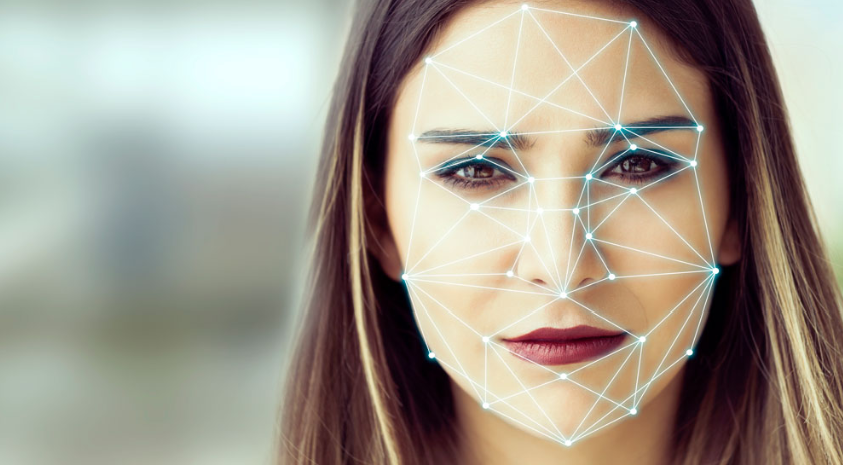
\includegraphics[width=3.46875in,height=\textheight]{Facial_Analysis.png}

\hypertarget{language-analysis}{%
\subsection{Language Analysis}\label{language-analysis}}

On the other hand, language analysis will focus on the content of your responses and the nature of your delivery. During or immediately after the recorded interview, the AI tool will convert your responses to text. Then, it'll parse through this and look for various things. From a content perspective, this may include the \textbf{technical language} and \textbf{vocabulary} you use that aligns with the job description and what the company is looking for (1). From a delivery perspective, this may include \textbf{active vs passive voice}, \textbf{run-on sentences}, the use of \textbf{filler words}, and the \textbf{tone} of your voice.

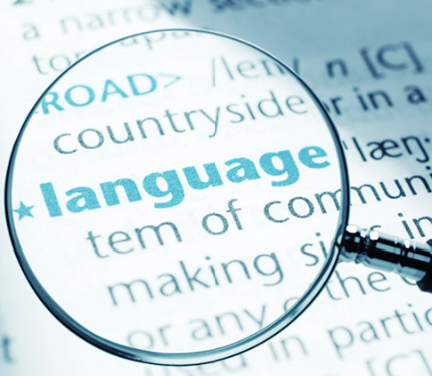
\includegraphics[width=2.16667in,height=\textheight]{Language_Analysis.png}

\hypertarget{benefits}{%
\section{Benefits}\label{benefits}}

AI-assessed interviews provide numerous benefits for both the recruiter and candidate:

\begin{itemize}
\item
  \textbf{Recruiters}

  \begin{itemize}
  \item
    Allows the company to accept more applicants to the open position~
  \item
    Spend less money on employees to assess the video recordings
  \item
    Removes the bottleneck of screening the recordings by hand
  \end{itemize}
\item
  \textbf{Candidates}

  \begin{itemize}
  \item
    While there is always a deadline, you can choose to do the recorded interview when it works best in your schedule
  \item
    More fair hiring process that isn't influenced as much by preconceptions and human biases and instead focuses more on qualifications
  \end{itemize}
\end{itemize}

\hypertarget{drawbacks}{%
\section{Drawbacks}\label{drawbacks}}

While AI-assessed interviews have its benefits, there are some significant drawbacks:

\begin{itemize}
\item
  AI tools must be coded by humans in the first place, so there is no guarantee that the tool will be free of human biases
\item
  They may reinforce discriminatory practices such as penalizing someone with a strong accent or speed impediment
\item
  Human emotions and facial expressions are very complex and may not be interpreted correctly, which can inadvertently remove a qualified candidate from the selection process
\item
  Concerns regarding personal privacy and data security due to the large amounts of information being collected during the recordings
\end{itemize}

\hypertarget{what-you-a-student-can-do}{%
\section{What You (A Student) Can Do!}\label{what-you-a-student-can-do}}

As a student preparing for the recruiting process this upcoming school year, you may be wondering how you can best set yourself up for success if you ever experience one of these AI interviews. \textbf{Look no further!} The following subsections highlight some tips and best practices.

\hypertarget{general-preparation}{%
\subsection{General Preparation}\label{general-preparation}}

General preparation relates to activities and preparation work you should be doing prior to the interview to ensure your best prepared to answer the questions.

\begin{itemize}
\item
  Research the company and general job type thoroughly in case of any questions related to why you want to work for the company or why you are applying to that positions
\item
  Prepare what you are going to say. Research some \href{https://www.themuse.com/advice/interview-questions-and-answers}{commonly asked interview questions} and make sure you have a story bank of your past experiences that you can pull from and adjust based on the question asked
\item
  Practice using the \href{https://www.themuse.com/advice/star-interview-method}{STAR (situation, task, action, result) method} as it's very popular framework for providing a response that is coherent, comprehensive, and insightful
\end{itemize}

\hypertarget{countering-the-ai-tools}{%
\subsection{Countering the AI Tools}\label{countering-the-ai-tools}}

Countering the AI tools relates to what you should do during the interview based on what the AI tools are looking for and analyzing.

\begin{itemize}
\item
  Practice talking to a camera and recording yourself so you get a good feel for where you're at and how to make progress (see Chapter 6: Student Practice Interviews)
\item
  Dress as if you were being interviewed by an actual interviewer in person
\item
  Clean the background of your recording space so the AI tool doesn't penalize you for a distracting background or make it harder for it to more accurately read your facial expressions
\item
  Ensure your lighting is good to allow for a proper facial analysis by the AI
\item
  Try to maintain eye contact with the camera as much as possible and use sticky notes on the computer/laptop if you want to refer to material
\item
  Keep your head high or at a neutral position; avoid angling your head downward
\item
  Smile and maintain a happy facial expression
\item
  Avoid the use of filler words like ``um'', ``like'', or ``hmm''
\item
  Use keywords (skills and job duties) from the job description during your responses if you can
\item
  Speak clearly and loudly (more than usual) to ensure the AI tool can translate your verbal response into text
\item
  Try not to furrow your eyebrows as it can be interpreted as confusion, disapproval, or worry
\end{itemize}

\hypertarget{skill-assessments}{%
\chapter{Skill Assessments}\label{skill-assessments}}

\hypertarget{predicting-candidates-success}{%
\chapter{Predicting Candidates' Success}\label{predicting-candidates-success}}

\hypertarget{conclusion}{%
\chapter{Conclusion}\label{conclusion}}

\hypertarget{our-working-process}{%
\chapter{Our Working Process}\label{our-working-process}}

\hypertarget{references}{%
\chapter{References}\label{references}}

\hypertarget{what-is-artificial-intelligence-ai-1}{%
\section{What is Artificial Intelligence (AI)?}\label{what-is-artificial-intelligence-ai-1}}

\begin{enumerate}
\def\labelenumi{(\arabic{enumi})}
\tightlist
\item
  \url{https://www.techtarget.com/searchenterpriseai/definition/AI-Artificial-Intelligence?Offer=abt_pubpro_AI-Insider}
\end{enumerate}

\hypertarget{ai-tools-for-job-searching-1}{%
\section{AI Tools for Job Searching}\label{ai-tools-for-job-searching-1}}

\hypertarget{resume-and-cover-letter-optimizer}{%
\section{Resume and Cover Letter Optimizer}\label{resume-and-cover-letter-optimizer}}

\hypertarget{student-practice-interview}{%
\section{Student Practice Interview}\label{student-practice-interview}}

\hypertarget{automated-applications-1}{%
\section{Automated Applications}\label{automated-applications-1}}

\hypertarget{what-are-applicant-tracking-systems-ats-1}{%
\section{What are Applicant Tracking Systems (ATS)?}\label{what-are-applicant-tracking-systems-ats-1}}

\hypertarget{recruiting-chatbots-1}{%
\section{Recruiting Chatbots}\label{recruiting-chatbots-1}}

\hypertarget{resume-and-cover-letter-screening-1}{%
\section{Resume and Cover Letter Screening}\label{resume-and-cover-letter-screening-1}}

\hypertarget{video-interview-assessments-1}{%
\section{Video Interview Assessments}\label{video-interview-assessments-1}}

\begin{enumerate}
\def\labelenumi{(\arabic{enumi})}
\item
  \url{https://www.hubert.ai/insights/what-are-ai-interviews\%5C}
\item
  \url{https://theconversation.com/facial-analysis-ai-is-being-used-in-job-interviews-it-will-probably-reinforce-inequality-124790}
\end{enumerate}

\hypertarget{skill-assessments-1}{%
\section{Skill Assessments}\label{skill-assessments-1}}

\hypertarget{predicting-candidates-success-1}{%
\section{Predicting Candidates' Success}\label{predicting-candidates-success-1}}

  \bibliography{book.bib,packages.bib}

\end{document}
